\documentclass[11]{article}
\usepackage{amsthm, amssymb, amsmath,verbatim}
\usepackage[margin=1in]{geometry}
\usepackage{enumerate}
\usepackage{enumitem}
\usepackage{graphicx}

\newtheorem*{claim}{Claim}
\newtheorem{ques}{Question}

\usepackage[T1]{fontenc}
    % Nicer default font (+ math font) than Computer Modern for most use cases
    \usepackage{mathpazo}

    % Basic figure setup, for now with no caption control since it's done
    % automatically by Pandoc (which extracts ![](path) syntax from Markdown).
    \usepackage{graphicx}
    % We will generate all images so they have a width \maxwidth. This means
    % that they will get their normal width if they fit onto the page, but
    % are scaled down if they would overflow the margins.
    \makeatletter
    \def\maxwidth{\ifdim\Gin@nat@width>\linewidth\linewidth
    \else\Gin@nat@width\fi}
    \makeatother
    \let\Oldincludegraphics\includegraphics
    % Set max figure width to be 80% of text width, for now hardcoded.
    \renewcommand{\includegraphics}[1]{\Oldincludegraphics[width=.8\maxwidth]{#1}}
    % Ensure that by default, figures have no caption (until we provide a
    % proper Figure object with a Caption API and a way to capture that
    % in the conversion process - todo).
    \usepackage{caption}
    \DeclareCaptionLabelFormat{nolabel}{}
    \captionsetup{labelformat=nolabel}

    \usepackage{adjustbox} % Used to constrain images to a maximum size 
    \usepackage{xcolor} % Allow colors to be defined
    \usepackage{enumerate} % Needed for markdown enumerations to work
    \usepackage{geometry} % Used to adjust the document margins
    \usepackage{amsmath} % Equations
    \usepackage{amssymb} % Equations
    \usepackage{textcomp} % defines textquotesingle
    % Hack from http://tex.stackexchange.com/a/47451/13684:
    \AtBeginDocument{%
        \def\PYZsq{\textquotesingle}% Upright quotes in Pygmentized code
    }
    \usepackage{upquote} % Upright quotes for verbatim code
    \usepackage{eurosym} % defines \euro
    \usepackage[mathletters]{ucs} % Extended unicode (utf-8) support
    \usepackage[utf8x]{inputenc} % Allow utf-8 characters in the tex document
    \usepackage{fancyvrb} % verbatim replacement that allows latex
    \usepackage{grffile} % extends the file name processing of package graphics 
                         % to support a larger range 
    % The hyperref package gives us a pdf with properly built
    % internal navigation ('pdf bookmarks' for the table of contents,
    % internal cross-reference links, web links for URLs, etc.)
    \usepackage{hyperref}
    \usepackage{longtable} % longtable support required by pandoc >1.10
    \usepackage{booktabs}  % table support for pandoc > 1.12.2

    

    
    
    % Colors for the hyperref package
    \definecolor{urlcolor}{rgb}{0,.145,.698}
    \definecolor{linkcolor}{rgb}{.71,0.21,0.01}
    \definecolor{citecolor}{rgb}{.12,.54,.11}

    % ANSI colors
    \definecolor{ansi-black}{HTML}{3E424D}
    \definecolor{ansi-black-intense}{HTML}{282C36}
    \definecolor{ansi-red}{HTML}{E75C58}
    \definecolor{ansi-red-intense}{HTML}{B22B31}
    \definecolor{ansi-green}{HTML}{00A250}
    \definecolor{ansi-green-intense}{HTML}{007427}
    \definecolor{ansi-yellow}{HTML}{DDB62B}
    \definecolor{ansi-yellow-intense}{HTML}{B27D12}
    \definecolor{ansi-blue}{HTML}{208FFB}
    \definecolor{ansi-blue-intense}{HTML}{0065CA}
    \definecolor{ansi-magenta}{HTML}{D160C4}
    \definecolor{ansi-magenta-intense}{HTML}{A03196}
    \definecolor{ansi-cyan}{HTML}{60C6C8}
    \definecolor{ansi-cyan-intense}{HTML}{258F8F}
    \definecolor{ansi-white}{HTML}{C5C1B4}
    \definecolor{ansi-white-intense}{HTML}{A1A6B2}

    % commands and environments needed by pandoc snippets
    % extracted from the output of `pandoc -s`
    \providecommand{\tightlist}{%
      \setlength{\itemsep}{0pt}\setlength{\parskip}{0pt}}
    \DefineVerbatimEnvironment{Highlighting}{Verbatim}{commandchars=\\\{\}}
    % Add ',fontsize=\small' for more characters per line
    \newenvironment{Shaded}{}{}
    \newcommand{\KeywordTok}[1]{\textcolor[rgb]{0.00,0.44,0.13}{\textbf{{#1}}}}
    \newcommand{\DataTypeTok}[1]{\textcolor[rgb]{0.56,0.13,0.00}{{#1}}}
    \newcommand{\DecValTok}[1]{\textcolor[rgb]{0.25,0.63,0.44}{{#1}}}
    \newcommand{\BaseNTok}[1]{\textcolor[rgb]{0.25,0.63,0.44}{{#1}}}
    \newcommand{\FloatTok}[1]{\textcolor[rgb]{0.25,0.63,0.44}{{#1}}}
    \newcommand{\CharTok}[1]{\textcolor[rgb]{0.25,0.44,0.63}{{#1}}}
    \newcommand{\StringTok}[1]{\textcolor[rgb]{0.25,0.44,0.63}{{#1}}}
    \newcommand{\CommentTok}[1]{\textcolor[rgb]{0.38,0.63,0.69}{\textit{{#1}}}}
    \newcommand{\OtherTok}[1]{\textcolor[rgb]{0.00,0.44,0.13}{{#1}}}
    \newcommand{\AlertTok}[1]{\textcolor[rgb]{1.00,0.00,0.00}{\textbf{{#1}}}}
    \newcommand{\FunctionTok}[1]{\textcolor[rgb]{0.02,0.16,0.49}{{#1}}}
    \newcommand{\RegionMarkerTok}[1]{{#1}}
    \newcommand{\ErrorTok}[1]{\textcolor[rgb]{1.00,0.00,0.00}{\textbf{{#1}}}}
    \newcommand{\NormalTok}[1]{{#1}}
    
    % Additional commands for more recent versions of Pandoc
    \newcommand{\ConstantTok}[1]{\textcolor[rgb]{0.53,0.00,0.00}{{#1}}}
    \newcommand{\SpecialCharTok}[1]{\textcolor[rgb]{0.25,0.44,0.63}{{#1}}}
    \newcommand{\VerbatimStringTok}[1]{\textcolor[rgb]{0.25,0.44,0.63}{{#1}}}
    \newcommand{\SpecialStringTok}[1]{\textcolor[rgb]{0.73,0.40,0.53}{{#1}}}
    \newcommand{\ImportTok}[1]{{#1}}
    \newcommand{\DocumentationTok}[1]{\textcolor[rgb]{0.73,0.13,0.13}{\textit{{#1}}}}
    \newcommand{\AnnotationTok}[1]{\textcolor[rgb]{0.38,0.63,0.69}{\textbf{\textit{{#1}}}}}
    \newcommand{\CommentVarTok}[1]{\textcolor[rgb]{0.38,0.63,0.69}{\textbf{\textit{{#1}}}}}
    \newcommand{\VariableTok}[1]{\textcolor[rgb]{0.10,0.09,0.49}{{#1}}}
    \newcommand{\ControlFlowTok}[1]{\textcolor[rgb]{0.00,0.44,0.13}{\textbf{{#1}}}}
    \newcommand{\OperatorTok}[1]{\textcolor[rgb]{0.40,0.40,0.40}{{#1}}}
    \newcommand{\BuiltInTok}[1]{{#1}}
    \newcommand{\ExtensionTok}[1]{{#1}}
    \newcommand{\PreprocessorTok}[1]{\textcolor[rgb]{0.74,0.48,0.00}{{#1}}}
    \newcommand{\AttributeTok}[1]{\textcolor[rgb]{0.49,0.56,0.16}{{#1}}}
    \newcommand{\InformationTok}[1]{\textcolor[rgb]{0.38,0.63,0.69}{\textbf{\textit{{#1}}}}}
    \newcommand{\WarningTok}[1]{\textcolor[rgb]{0.38,0.63,0.69}{\textbf{\textit{{#1}}}}}
    
    
    % Define a nice break command that doesn't care if a line doesn't already
    % exist.
    \def\br{\hspace*{\fill} \\* }
    % Math Jax compatability definitions
    \def\gt{>}
    \def\lt{<}
    
    
    

    % Pygments definitions
    
\makeatletter
\def\PY@reset{\let\PY@it=\relax \let\PY@bf=\relax%
    \let\PY@ul=\relax \let\PY@tc=\relax%
    \let\PY@bc=\relax \let\PY@ff=\relax}
\def\PY@tok#1{\csname PY@tok@#1\endcsname}
\def\PY@toks#1+{\ifx\relax#1\empty\else%
    \PY@tok{#1}\expandafter\PY@toks\fi}
\def\PY@do#1{\PY@bc{\PY@tc{\PY@ul{%
    \PY@it{\PY@bf{\PY@ff{#1}}}}}}}
\def\PY#1#2{\PY@reset\PY@toks#1+\relax+\PY@do{#2}}

\expandafter\def\csname PY@tok@w\endcsname{\def\PY@tc##1{\textcolor[rgb]{0.73,0.73,0.73}{##1}}}
\expandafter\def\csname PY@tok@c\endcsname{\let\PY@it=\textit\def\PY@tc##1{\textcolor[rgb]{0.25,0.50,0.50}{##1}}}
\expandafter\def\csname PY@tok@cp\endcsname{\def\PY@tc##1{\textcolor[rgb]{0.74,0.48,0.00}{##1}}}
\expandafter\def\csname PY@tok@k\endcsname{\let\PY@bf=\textbf\def\PY@tc##1{\textcolor[rgb]{0.00,0.50,0.00}{##1}}}
\expandafter\def\csname PY@tok@kp\endcsname{\def\PY@tc##1{\textcolor[rgb]{0.00,0.50,0.00}{##1}}}
\expandafter\def\csname PY@tok@kt\endcsname{\def\PY@tc##1{\textcolor[rgb]{0.69,0.00,0.25}{##1}}}
\expandafter\def\csname PY@tok@o\endcsname{\def\PY@tc##1{\textcolor[rgb]{0.40,0.40,0.40}{##1}}}
\expandafter\def\csname PY@tok@ow\endcsname{\let\PY@bf=\textbf\def\PY@tc##1{\textcolor[rgb]{0.67,0.13,1.00}{##1}}}
\expandafter\def\csname PY@tok@nb\endcsname{\def\PY@tc##1{\textcolor[rgb]{0.00,0.50,0.00}{##1}}}
\expandafter\def\csname PY@tok@nf\endcsname{\def\PY@tc##1{\textcolor[rgb]{0.00,0.00,1.00}{##1}}}
\expandafter\def\csname PY@tok@nc\endcsname{\let\PY@bf=\textbf\def\PY@tc##1{\textcolor[rgb]{0.00,0.00,1.00}{##1}}}
\expandafter\def\csname PY@tok@nn\endcsname{\let\PY@bf=\textbf\def\PY@tc##1{\textcolor[rgb]{0.00,0.00,1.00}{##1}}}
\expandafter\def\csname PY@tok@ne\endcsname{\let\PY@bf=\textbf\def\PY@tc##1{\textcolor[rgb]{0.82,0.25,0.23}{##1}}}
\expandafter\def\csname PY@tok@nv\endcsname{\def\PY@tc##1{\textcolor[rgb]{0.10,0.09,0.49}{##1}}}
\expandafter\def\csname PY@tok@no\endcsname{\def\PY@tc##1{\textcolor[rgb]{0.53,0.00,0.00}{##1}}}
\expandafter\def\csname PY@tok@nl\endcsname{\def\PY@tc##1{\textcolor[rgb]{0.63,0.63,0.00}{##1}}}
\expandafter\def\csname PY@tok@ni\endcsname{\let\PY@bf=\textbf\def\PY@tc##1{\textcolor[rgb]{0.60,0.60,0.60}{##1}}}
\expandafter\def\csname PY@tok@na\endcsname{\def\PY@tc##1{\textcolor[rgb]{0.49,0.56,0.16}{##1}}}
\expandafter\def\csname PY@tok@nt\endcsname{\let\PY@bf=\textbf\def\PY@tc##1{\textcolor[rgb]{0.00,0.50,0.00}{##1}}}
\expandafter\def\csname PY@tok@nd\endcsname{\def\PY@tc##1{\textcolor[rgb]{0.67,0.13,1.00}{##1}}}
\expandafter\def\csname PY@tok@s\endcsname{\def\PY@tc##1{\textcolor[rgb]{0.73,0.13,0.13}{##1}}}
\expandafter\def\csname PY@tok@sd\endcsname{\let\PY@it=\textit\def\PY@tc##1{\textcolor[rgb]{0.73,0.13,0.13}{##1}}}
\expandafter\def\csname PY@tok@si\endcsname{\let\PY@bf=\textbf\def\PY@tc##1{\textcolor[rgb]{0.73,0.40,0.53}{##1}}}
\expandafter\def\csname PY@tok@se\endcsname{\let\PY@bf=\textbf\def\PY@tc##1{\textcolor[rgb]{0.73,0.40,0.13}{##1}}}
\expandafter\def\csname PY@tok@sr\endcsname{\def\PY@tc##1{\textcolor[rgb]{0.73,0.40,0.53}{##1}}}
\expandafter\def\csname PY@tok@ss\endcsname{\def\PY@tc##1{\textcolor[rgb]{0.10,0.09,0.49}{##1}}}
\expandafter\def\csname PY@tok@sx\endcsname{\def\PY@tc##1{\textcolor[rgb]{0.00,0.50,0.00}{##1}}}
\expandafter\def\csname PY@tok@m\endcsname{\def\PY@tc##1{\textcolor[rgb]{0.40,0.40,0.40}{##1}}}
\expandafter\def\csname PY@tok@gh\endcsname{\let\PY@bf=\textbf\def\PY@tc##1{\textcolor[rgb]{0.00,0.00,0.50}{##1}}}
\expandafter\def\csname PY@tok@gu\endcsname{\let\PY@bf=\textbf\def\PY@tc##1{\textcolor[rgb]{0.50,0.00,0.50}{##1}}}
\expandafter\def\csname PY@tok@gd\endcsname{\def\PY@tc##1{\textcolor[rgb]{0.63,0.00,0.00}{##1}}}
\expandafter\def\csname PY@tok@gi\endcsname{\def\PY@tc##1{\textcolor[rgb]{0.00,0.63,0.00}{##1}}}
\expandafter\def\csname PY@tok@gr\endcsname{\def\PY@tc##1{\textcolor[rgb]{1.00,0.00,0.00}{##1}}}
\expandafter\def\csname PY@tok@ge\endcsname{\let\PY@it=\textit}
\expandafter\def\csname PY@tok@gs\endcsname{\let\PY@bf=\textbf}
\expandafter\def\csname PY@tok@gp\endcsname{\let\PY@bf=\textbf\def\PY@tc##1{\textcolor[rgb]{0.00,0.00,0.50}{##1}}}
\expandafter\def\csname PY@tok@go\endcsname{\def\PY@tc##1{\textcolor[rgb]{0.53,0.53,0.53}{##1}}}
\expandafter\def\csname PY@tok@gt\endcsname{\def\PY@tc##1{\textcolor[rgb]{0.00,0.27,0.87}{##1}}}
\expandafter\def\csname PY@tok@err\endcsname{\def\PY@bc##1{\setlength{\fboxsep}{0pt}\fcolorbox[rgb]{1.00,0.00,0.00}{1,1,1}{\strut ##1}}}
\expandafter\def\csname PY@tok@kc\endcsname{\let\PY@bf=\textbf\def\PY@tc##1{\textcolor[rgb]{0.00,0.50,0.00}{##1}}}
\expandafter\def\csname PY@tok@kd\endcsname{\let\PY@bf=\textbf\def\PY@tc##1{\textcolor[rgb]{0.00,0.50,0.00}{##1}}}
\expandafter\def\csname PY@tok@kn\endcsname{\let\PY@bf=\textbf\def\PY@tc##1{\textcolor[rgb]{0.00,0.50,0.00}{##1}}}
\expandafter\def\csname PY@tok@kr\endcsname{\let\PY@bf=\textbf\def\PY@tc##1{\textcolor[rgb]{0.00,0.50,0.00}{##1}}}
\expandafter\def\csname PY@tok@bp\endcsname{\def\PY@tc##1{\textcolor[rgb]{0.00,0.50,0.00}{##1}}}
\expandafter\def\csname PY@tok@fm\endcsname{\def\PY@tc##1{\textcolor[rgb]{0.00,0.00,1.00}{##1}}}
\expandafter\def\csname PY@tok@vc\endcsname{\def\PY@tc##1{\textcolor[rgb]{0.10,0.09,0.49}{##1}}}
\expandafter\def\csname PY@tok@vg\endcsname{\def\PY@tc##1{\textcolor[rgb]{0.10,0.09,0.49}{##1}}}
\expandafter\def\csname PY@tok@vi\endcsname{\def\PY@tc##1{\textcolor[rgb]{0.10,0.09,0.49}{##1}}}
\expandafter\def\csname PY@tok@vm\endcsname{\def\PY@tc##1{\textcolor[rgb]{0.10,0.09,0.49}{##1}}}
\expandafter\def\csname PY@tok@sa\endcsname{\def\PY@tc##1{\textcolor[rgb]{0.73,0.13,0.13}{##1}}}
\expandafter\def\csname PY@tok@sb\endcsname{\def\PY@tc##1{\textcolor[rgb]{0.73,0.13,0.13}{##1}}}
\expandafter\def\csname PY@tok@sc\endcsname{\def\PY@tc##1{\textcolor[rgb]{0.73,0.13,0.13}{##1}}}
\expandafter\def\csname PY@tok@dl\endcsname{\def\PY@tc##1{\textcolor[rgb]{0.73,0.13,0.13}{##1}}}
\expandafter\def\csname PY@tok@s2\endcsname{\def\PY@tc##1{\textcolor[rgb]{0.73,0.13,0.13}{##1}}}
\expandafter\def\csname PY@tok@sh\endcsname{\def\PY@tc##1{\textcolor[rgb]{0.73,0.13,0.13}{##1}}}
\expandafter\def\csname PY@tok@s1\endcsname{\def\PY@tc##1{\textcolor[rgb]{0.73,0.13,0.13}{##1}}}
\expandafter\def\csname PY@tok@mb\endcsname{\def\PY@tc##1{\textcolor[rgb]{0.40,0.40,0.40}{##1}}}
\expandafter\def\csname PY@tok@mf\endcsname{\def\PY@tc##1{\textcolor[rgb]{0.40,0.40,0.40}{##1}}}
\expandafter\def\csname PY@tok@mh\endcsname{\def\PY@tc##1{\textcolor[rgb]{0.40,0.40,0.40}{##1}}}
\expandafter\def\csname PY@tok@mi\endcsname{\def\PY@tc##1{\textcolor[rgb]{0.40,0.40,0.40}{##1}}}
\expandafter\def\csname PY@tok@il\endcsname{\def\PY@tc##1{\textcolor[rgb]{0.40,0.40,0.40}{##1}}}
\expandafter\def\csname PY@tok@mo\endcsname{\def\PY@tc##1{\textcolor[rgb]{0.40,0.40,0.40}{##1}}}
\expandafter\def\csname PY@tok@ch\endcsname{\let\PY@it=\textit\def\PY@tc##1{\textcolor[rgb]{0.25,0.50,0.50}{##1}}}
\expandafter\def\csname PY@tok@cm\endcsname{\let\PY@it=\textit\def\PY@tc##1{\textcolor[rgb]{0.25,0.50,0.50}{##1}}}
\expandafter\def\csname PY@tok@cpf\endcsname{\let\PY@it=\textit\def\PY@tc##1{\textcolor[rgb]{0.25,0.50,0.50}{##1}}}
\expandafter\def\csname PY@tok@c1\endcsname{\let\PY@it=\textit\def\PY@tc##1{\textcolor[rgb]{0.25,0.50,0.50}{##1}}}
\expandafter\def\csname PY@tok@cs\endcsname{\let\PY@it=\textit\def\PY@tc##1{\textcolor[rgb]{0.25,0.50,0.50}{##1}}}

\def\PYZbs{\char`\\}
\def\PYZus{\char`\_}
\def\PYZob{\char`\{}
\def\PYZcb{\char`\}}
\def\PYZca{\char`\^}
\def\PYZam{\char`\&}
\def\PYZlt{\char`\<}
\def\PYZgt{\char`\>}
\def\PYZsh{\char`\#}
\def\PYZpc{\char`\%}
\def\PYZdl{\char`\$}
\def\PYZhy{\char`\-}
\def\PYZsq{\char`\'}
\def\PYZdq{\char`\"}
\def\PYZti{\char`\~}
% for compatibility with earlier versions
\def\PYZat{@}
\def\PYZlb{[}
\def\PYZrb{]}
\makeatother


    % Exact colors from NB
    \definecolor{incolor}{rgb}{0.0, 0.0, 0.5}
    \definecolor{outcolor}{rgb}{0.545, 0.0, 0.0}



    
    % Prevent overflowing lines due to hard-to-break entities
    \sloppy 
    % Setup hyperref package
    \hypersetup{
      breaklinks=true,  % so long urls are correctly broken across lines
      colorlinks=true,
      urlcolor=urlcolor,
      linkcolor=linkcolor,
      citecolor=citecolor,
      }
    % Slightly bigger margins than the latex defaults
    
    \geometry{verbose,tmargin=1in,bmargin=1in,lmargin=1in,rmargin=1in}

\title{CSE 150 Homework 4}
\date{Fall 2018}
\author{Pedro Sousa Meireles\\ A15677282}
\begin{document}

\maketitle
\section{Maximum Likelihood Estimation}
$$P_{ML}(X_i=x|pa_i=\pi)=\frac{count(X_i=x,pa_i=\pi)}{\sum_{x'}count(X_i=x',pa_i=\pi)}$$
\begin{enumerate}[label=(\alph*)]
\item
$$P(Y=y)=\frac{count(Y=y)}{T}$$
$$P(X=x|Y=y)=\frac{count(X=x,Y=y)}{count(Y=y)}$$
$$P(Z=x|Y=y)=\frac{count(Y=y,Z=z)}{count(Y=y)}$$
\item
$$P(Z=z)=\frac{count(Z=z)}{T}$$
$$P(Y=y|Z=z)=\frac{count(Y=y,Z=z)}{count(Z=z)}$$
$$P(X=x|Y=y)=\frac{count(X=x,Y=y)}{count(Y=y)}$$
\item
Left DAG:
\begin{align*}
P(X=x, Y=y, Z=z)&=P(Y=y) \cdot P(X=x|Y=y) \cdot P(Z=z|Y=y)\\
&=\frac{count(Y=y)}{T} \cdot \frac{count(X=x,Y=y)}{count(Y=y)} \cdot \frac{count(Y=y,Z=z)}{count(Y=y)}\\
&=\frac{count(X=x,Y=y) \cdot count(Y=y,Z=z)}{T \cdot count(Y=y)}
\end{align*}

Right DAG:
\begin{align*}
P(X=x, Y=y, Z=z)&=P(Z=z) \cdot P(Y=y|Z=z) \cdot P(X=x|Y=y)\\
&=\frac{count(Z=z)}{T} \cdot \frac{count(Y=y,Z=z)}{count(Z=z)} \cdot \frac{count(X=x,Y=y)}{count(Y=y)}\\
&=\frac{count(X=x,Y=y) \cdot count(Y=y,Z=z)}{T \cdot count(Y=y)}
\end{align*}

\item
No. Every conditional independence implied by one graph is also present in the other. The only variables that are conditional independent are X and Z given Y. All other combination of variables are conditionally dependent. Given that both graphs gave the same conditional independence relations it is consistent with the result of item C.
\end{enumerate}
\pagebreak

\section{Survey}
Done

\section{Statistical language modeling}
\begin{enumerate}[label=(\alph*)]
\item
\begin{center}
\begin{tabular}{|c|c|}
\hline
\textbf{$w$} & \textbf{$P_u(w)$}      \\ \hline
NINETEEN     & 0.0028588174836726445  \\ \hline
NOT          & 0.0021457733600835156  \\ \hline
NEW          & 0.001900350279776441   \\ \hline
NINE         & 0.0017613053303564415  \\ \hline
NINETY       & 0.0012920576727483372  \\ \hline
NO           & 0.0010485914217056834  \\ \hline
NOW          & 0.0007126160671875371  \\ \hline
N.           & 0.0006647838218553515  \\ \hline
NATIONAL     & 0.0005965149408928713  \\ \hline
NEXT         & 0.00042879021256620473 \\ \hline
NEWS         & 0.0004290959671387705  \\ \hline
NUMBER       & 0.0003488781974804209  \\ \hline
NORTH        & 0.0002554640604701336  \\ \hline
NEVER        & 0.0002425367571420538  \\ \hline
NIGHT        & 0.00023650727697105726 \\ \hline
NEARLY       & 0.0002124871977502921  \\ \hline
NEAR         & 0.00021042029683974764 \\ \hline
NEED         & 0.00020837785629500844 \\ \hline
\end{tabular}
\end{center}

\item
\begin{center}
\begin{tabular}{|c|c|}
\hline
\textbf{$w'$} & \textbf{$P_u(w'|w=HAVE)$} \\ \hline
$<$UNK$>$         & 0.4116813942572601        \\ \hline
BEEN          & 0.17246178649415317       \\ \hline
TO            & 0.08213301769351646       \\ \hline
A             & 0.06311299769392462       \\ \hline
THE           & 0.028934103385645192      \\ \hline
NO            & 0.015738454317258833      \\ \hline
NOT           & 0.01344462357911063       \\ \hline
SAID          & 0.013040550192853207      \\ \hline
HAD           & 0.01128956551907104       \\ \hline
AN            & 0.010897736780882022      \\ \hline
\end{tabular}
\end{center}

\item
$$L_u=-50.562145130091004$$
$$L_b=-43.04832187498447$$

The bigram model yields the highest log-likelihood.
\item
$$L_u=-44.72653897141283$$
$$L_b=-\infty$$

The pairs of adjacent words that are not observed in the corpus are (RECENT $\rightarrow$ OFFICIALS) and (INCORPORATED $\rightarrow$ PRICES). Since $P(word|evidence)=0$ when there is no observation in the corpus, the total probability is 0, which makes the log-likelihood approach $-\infty$, because 0 is not in log function domain.

\item
\begin{figure}
\centering
  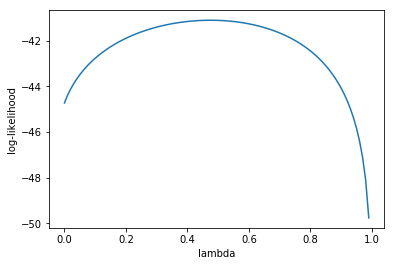
\includegraphics{log-likelihood.png}
\end{figure}

The optimal value of $\lambda$ is 0.48.
\item

\begin{Verbatim}[commandchars=\\\{\}]
{\color{incolor}In [{\color{incolor}1}]:} \PY{n}{words} \PY{o}{=} \PY{p}{[}\PY{p}{]}
        \PY{k}{for} \PY{n}{line} \PY{o+ow}{in} \PY{n+nb}{open}\PY{p}{(}\PY{l+s+s2}{\PYZdq{}}\PY{l+s+s2}{hw4\PYZus{}vocab.txt}\PY{l+s+s2}{\PYZdq{}}\PY{p}{)}\PY{p}{:}
          \PY{n}{words}\PY{o}{.}\PY{n}{append}\PY{p}{(}\PY{n}{line}\PY{o}{.}\PY{n}{split}\PY{p}{(}\PY{p}{)}\PY{p}{[}\PY{l+m+mi}{0}\PY{p}{]}\PY{p}{)}
        
        \PY{n}{counts} \PY{o}{=} \PY{p}{[}\PY{p}{]}
        \PY{k}{for} \PY{n}{line} \PY{o+ow}{in} \PY{n+nb}{open}\PY{p}{(}\PY{l+s+s2}{\PYZdq{}}\PY{l+s+s2}{hw4\PYZus{}unigram.txt}\PY{l+s+s2}{\PYZdq{}}\PY{p}{)}\PY{p}{:}
          \PY{n}{counts}\PY{o}{.}\PY{n}{append}\PY{p}{(}\PY{n+nb}{int}\PY{p}{(}\PY{n}{line}\PY{o}{.}\PY{n}{split}\PY{p}{(}\PY{p}{)}\PY{p}{[}\PY{l+m+mi}{0}\PY{p}{]}\PY{p}{)}\PY{p}{)}
        
        \PY{n}{bigram} \PY{o}{=} \PY{p}{[}\PY{p}{]}
        \PY{k}{for} \PY{n}{line} \PY{o+ow}{in} \PY{n+nb}{open}\PY{p}{(}\PY{l+s+s2}{\PYZdq{}}\PY{l+s+s2}{hw4\PYZus{}bigram.txt}\PY{l+s+s2}{\PYZdq{}}\PY{p}{)}\PY{p}{:}
          \PY{n}{bigram}\PY{o}{.}\PY{n}{append}\PY{p}{(}\PY{p}{[}\PY{n+nb}{int} \PY{p}{(}\PY{n}{x}\PY{p}{)} \PY{k}{for} \PY{n}{x} \PY{o+ow}{in} \PY{n}{line}\PY{o}{.}\PY{n}{split}\PY{p}{(}\PY{p}{)}\PY{p}{]}\PY{p}{)}
\end{Verbatim}


    \begin{Verbatim}[commandchars=\\\{\}]
{\color{incolor}In [{\color{incolor}2}]:} \PY{n}{unigram} \PY{o}{=} \PY{n+nb}{list}\PY{p}{(}\PY{n+nb}{zip}\PY{p}{(}\PY{n}{words}\PY{p}{,} \PY{n}{counts}\PY{p}{)}\PY{p}{)}
\end{Verbatim}


    \subsection{(a)}\label{a}

    \begin{Verbatim}[commandchars=\\\{\}]
{\color{incolor}In [{\color{incolor}3}]:} \PY{n}{probabilities} \PY{o}{=} \PY{p}{[}\PY{p}{]}
        \PY{k}{for} \PY{n}{i} \PY{o+ow}{in} \PY{n+nb}{range}\PY{p}{(}\PY{l+m+mi}{0}\PY{p}{,} \PY{l+m+mi}{499}\PY{p}{)}\PY{p}{:}
            \PY{n}{probabilities}\PY{o}{.}\PY{n}{append}\PY{p}{(}\PY{p}{[}\PY{n}{words}\PY{p}{[}\PY{n}{i}\PY{p}{]}\PY{p}{,} \PY{n}{counts}\PY{p}{[}\PY{n}{i}\PY{p}{]}\PY{o}{/}\PY{n+nb}{sum}\PY{p}{(}\PY{n}{counts}\PY{p}{)}\PY{p}{]}\PY{p}{)}
\end{Verbatim}


    \begin{Verbatim}[commandchars=\\\{\}]
{\color{incolor}In [{\color{incolor}4}]:} \PY{p}{[}\PY{n}{v} \PY{k}{for} \PY{n}{v} \PY{o+ow}{in} \PY{n}{probabilities} \PY{k}{if} \PY{n}{v}\PY{p}{[}\PY{l+m+mi}{0}\PY{p}{]}\PY{p}{[}\PY{l+m+mi}{0}\PY{p}{]} \PY{o}{==} \PY{l+s+s1}{\PYZsq{}}\PY{l+s+s1}{N}\PY{l+s+s1}{\PYZsq{}} \PY{o+ow}{or} \PY{n}{v}\PY{p}{[}\PY{l+m+mi}{0}\PY{p}{]}\PY{p}{[}\PY{l+m+mi}{0}\PY{p}{]} \PY{o}{==} \PY{l+s+s1}{\PYZsq{}}\PY{l+s+s1}{n}\PY{l+s+s1}{\PYZsq{}}\PY{p}{]}
\end{Verbatim}


\begin{Verbatim}[commandchars=\\\{\}]
{\color{outcolor}Out[{\color{outcolor}4}]:} [['NINETEEN', 0.0028588174836726445],
         ['NOT', 0.0021457733600835156],
         ['NEW', 0.001900350279776441],
         ['NINE', 0.0017613053303564415],
         ['NINETY', 0.0012920576727483372],
         ['NO', 0.0010485914217056834],
         ['NOW', 0.0007126160671875371],
         ['N.', 0.0006647838218553515],
         ['NATIONAL', 0.0005965149408928713],
         ['NEXT', 0.00042879021256620473],
         ['NEWS', 0.0004290959671387705],
         ['NUMBER', 0.0003488781974804209],
         ['NORTH', 0.0002554640604701336],
         ['NEVER', 0.0002425367571420538],
         ['NIGHT', 0.00023650727697105726],
         ['NEARLY', 0.0002124871977502921],
         ['NEAR', 0.00021042029683974764],
         ['NEED', 0.00020837785629500844]]
\end{Verbatim}
            
    \subsection{(b)}\label{b}

    \begin{Verbatim}[commandchars=\\\{\}]
{\color{incolor}In [{\color{incolor}5}]:} \PY{n}{words}\PY{p}{[}\PY{l+m+mi}{35}\PY{p}{]}
\end{Verbatim}


\begin{Verbatim}[commandchars=\\\{\}]
{\color{outcolor}Out[{\color{outcolor}5}]:} 'HAVE'
\end{Verbatim}
            
    \begin{Verbatim}[commandchars=\\\{\}]
{\color{incolor}In [{\color{incolor}6}]:} \PY{n}{biDist} \PY{o}{=} \PY{p}{[}\PY{p}{[}\PY{n}{words}\PY{p}{[}\PY{n}{v}\PY{p}{[}\PY{l+m+mi}{1}\PY{p}{]}\PY{o}{\PYZhy{}}\PY{l+m+mi}{1}\PY{p}{]}\PY{p}{,}\PY{n}{v}\PY{p}{[}\PY{l+m+mi}{2}\PY{p}{]}\PY{p}{]} \PY{k}{for} \PY{n}{v} \PY{o+ow}{in} \PY{n}{bigram} \PY{k}{if} \PY{n}{v}\PY{p}{[}\PY{l+m+mi}{0}\PY{p}{]} \PY{o}{==} \PY{l+m+mi}{36}\PY{p}{]}
\end{Verbatim}


    \begin{Verbatim}[commandchars=\\\{\}]
{\color{incolor}In [{\color{incolor}7}]:} \PY{n}{s} \PY{o}{=} \PY{n+nb}{sum}\PY{p}{(}\PY{p}{[}\PY{n}{v}\PY{p}{[}\PY{l+m+mi}{1}\PY{p}{]} \PY{k}{for} \PY{n}{v} \PY{o+ow}{in} \PY{n}{biDist}\PY{p}{]}\PY{p}{)}
        \PY{n}{biDist} \PY{o}{=} \PY{p}{[}\PY{p}{[}\PY{n}{v}\PY{p}{[}\PY{l+m+mi}{0}\PY{p}{]}\PY{p}{,}\PY{n}{v}\PY{p}{[}\PY{l+m+mi}{1}\PY{p}{]}\PY{o}{/}\PY{n}{s}\PY{p}{]} \PY{k}{for} \PY{n}{v} \PY{o+ow}{in} \PY{n}{biDist}\PY{p}{]}
\end{Verbatim}


    \begin{Verbatim}[commandchars=\\\{\}]
{\color{incolor}In [{\color{incolor}8}]:} \PY{n}{biDist} \PY{o}{=} \PY{n+nb}{sorted}\PY{p}{(}\PY{n}{biDist}\PY{p}{,} \PY{n}{key}\PY{o}{=}\PY{k}{lambda} \PY{n}{x}\PY{p}{:} \PY{n}{x}\PY{p}{[}\PY{l+m+mi}{1}\PY{p}{]}\PY{p}{)}
\end{Verbatim}


    \begin{Verbatim}[commandchars=\\\{\}]
{\color{incolor}In [{\color{incolor}9}]:} \PY{n}{biDist}\PY{p}{[}\PY{o}{\PYZhy{}}\PY{l+m+mi}{10}\PY{p}{:}\PY{p}{]}
\end{Verbatim}


\begin{Verbatim}[commandchars=\\\{\}]
{\color{outcolor}Out[{\color{outcolor}9}]:} [['AN', 0.010897736780882022],
         ['HAD', 0.01128956551907104],
         ['SAID', 0.013040550192853207],
         ['NOT', 0.01344462357911063],
         ['NO', 0.015738454317258833],
         ['THE', 0.028934103385645192],
         ['A', 0.06311299769392462],
         ['TO', 0.08213301769351646],
         ['BEEN', 0.17246178649415317],
         ['<UNK>', 0.4116813942572601]]
\end{Verbatim}
            
    \subsection{(c)}\label{c}

    \begin{Verbatim}[commandchars=\\\{\}]
{\color{incolor}In [{\color{incolor}10}]:} \PY{k+kn}{import} \PY{n+nn}{math}
         
         \PY{k}{def} \PY{n+nf}{probUnigram}\PY{p}{(}\PY{n}{word}\PY{p}{)}\PY{p}{:}
             \PY{k}{return} \PY{n}{probabilities}\PY{p}{[}\PY{n}{words}\PY{o}{.}\PY{n}{index}\PY{p}{(}\PY{n}{word}\PY{p}{)}\PY{p}{]}\PY{p}{[}\PY{l+m+mi}{1}\PY{p}{]}
         
         \PY{k}{def} \PY{n+nf}{probBigram}\PY{p}{(}\PY{n}{word}\PY{p}{,} \PY{n}{evidence}\PY{p}{)}\PY{p}{:}
             \PY{n}{dist} \PY{o}{=} \PY{p}{[}\PY{p}{[}\PY{n}{words}\PY{p}{[}\PY{n}{v}\PY{p}{[}\PY{l+m+mi}{1}\PY{p}{]}\PY{o}{\PYZhy{}}\PY{l+m+mi}{1}\PY{p}{]}\PY{p}{,}\PY{n}{v}\PY{p}{[}\PY{l+m+mi}{2}\PY{p}{]}\PY{p}{]} \PY{k}{for} \PY{n}{v} \PY{o+ow}{in} \PY{n}{bigram} \PY{k}{if} \PY{n}{v}\PY{p}{[}\PY{l+m+mi}{0}\PY{p}{]} \PY{o}{==} \PY{n}{words}\PY{o}{.}\PY{n}{index}\PY{p}{(}\PY{n}{evidence}\PY{p}{)}\PY{o}{+}\PY{l+m+mi}{1}\PY{p}{]}
             \PY{n}{psum} \PY{o}{=} \PY{n+nb}{sum}\PY{p}{(}\PY{p}{[}\PY{n}{v}\PY{p}{[}\PY{l+m+mi}{1}\PY{p}{]} \PY{k}{for} \PY{n}{v} \PY{o+ow}{in} \PY{n}{dist}\PY{p}{]}\PY{p}{)}
             \PY{n}{prob} \PY{o}{=} \PY{p}{[}\PY{n}{v}\PY{p}{[}\PY{l+m+mi}{1}\PY{p}{]} \PY{k}{for} \PY{n}{v} \PY{o+ow}{in} \PY{n}{dist} \PY{k}{if} \PY{n}{v}\PY{p}{[}\PY{l+m+mi}{0}\PY{p}{]} \PY{o}{==} \PY{n}{word}\PY{p}{]}
             \PY{k}{if} \PY{n+nb}{len}\PY{p}{(}\PY{n}{prob}\PY{p}{)} \PY{o}{==} \PY{l+m+mi}{0}\PY{p}{:}
                 \PY{k}{return} \PY{l+m+mi}{0}
             \PY{k}{else}\PY{p}{:}
                 \PY{k}{return} \PY{n}{prob}\PY{p}{[}\PY{l+m+mi}{0}\PY{p}{]}\PY{o}{/}\PY{n}{psum}
\end{Verbatim}


    \begin{Verbatim}[commandchars=\\\{\}]
{\color{incolor}In [{\color{incolor}11}]:} \PY{k}{def} \PY{n+nf}{logLikelihoods}\PY{p}{(}\PY{n}{sentence}\PY{p}{)}\PY{p}{:}
             \PY{n}{lu} \PY{o}{=} \PY{l+m+mi}{1}
             \PY{n}{lb} \PY{o}{=} \PY{l+m+mi}{1}
             \PY{n}{sent} \PY{o}{=} \PY{n}{sentence}\PY{o}{.}\PY{n}{split}\PY{p}{(}\PY{p}{)}
         
             \PY{k}{for} \PY{n}{i} \PY{o+ow}{in} \PY{n+nb}{range}\PY{p}{(}\PY{l+m+mi}{0}\PY{p}{,} \PY{n+nb}{len}\PY{p}{(}\PY{n}{sent}\PY{p}{)}\PY{p}{)}\PY{p}{:}
                 \PY{n}{lu} \PY{o}{=} \PY{n}{lu} \PY{o}{*} \PY{n}{probUnigram}\PY{p}{(}\PY{n}{sent}\PY{p}{[}\PY{n}{i}\PY{p}{]}\PY{p}{)}
                 \PY{k}{if} \PY{n}{i} \PY{o}{==} \PY{l+m+mi}{0}\PY{p}{:}
                     \PY{n}{lb} \PY{o}{=} \PY{n}{lb} \PY{o}{*} \PY{n}{probBigram}\PY{p}{(}\PY{n}{sent}\PY{p}{[}\PY{n}{i}\PY{p}{]}\PY{p}{,} \PY{l+s+s2}{\PYZdq{}}\PY{l+s+s2}{\PYZlt{}s\PYZgt{}}\PY{l+s+s2}{\PYZdq{}}\PY{p}{)}
                 \PY{k}{else}\PY{p}{:}
                     \PY{n}{lb} \PY{o}{=} \PY{n}{lb} \PY{o}{*} \PY{n}{probBigram}\PY{p}{(}\PY{n}{sent}\PY{p}{[}\PY{n}{i}\PY{p}{]}\PY{p}{,} \PY{n}{sent}\PY{p}{[}\PY{n}{i}\PY{o}{\PYZhy{}}\PY{l+m+mi}{1}\PY{p}{]}\PY{p}{)}
             \PY{k}{if} \PY{n}{lu} \PY{o}{!=} \PY{l+m+mi}{0}\PY{p}{:}
                 \PY{n}{lu} \PY{o}{=} \PY{n}{math}\PY{o}{.}\PY{n}{log}\PY{p}{(}\PY{n}{lu}\PY{p}{)}
             \PY{k}{else}\PY{p}{:}
                 \PY{n}{lu} \PY{o}{=} \PY{l+s+s2}{\PYZdq{}}\PY{l+s+s2}{UNDEFINED}\PY{l+s+s2}{\PYZdq{}}
             
             \PY{k}{if} \PY{n}{lb} \PY{o}{!=} \PY{l+m+mi}{0}\PY{p}{:}
                 \PY{n}{lb} \PY{o}{=} \PY{n}{math}\PY{o}{.}\PY{n}{log}\PY{p}{(}\PY{n}{lb}\PY{p}{)}
             \PY{k}{else}\PY{p}{:}
                 \PY{n}{lb} \PY{o}{=} \PY{l+s+s2}{\PYZdq{}}\PY{l+s+s2}{UNDEFINED}\PY{l+s+s2}{\PYZdq{}}
             \PY{k}{return} \PY{n}{lu}\PY{p}{,} \PY{n}{lb}
             
\end{Verbatim}


    \begin{Verbatim}[commandchars=\\\{\}]
{\color{incolor}In [{\color{incolor}12}]:} \PY{n}{lu}\PY{p}{,} \PY{n}{lb} \PY{o}{=} \PY{n}{logLikelihoods}\PY{p}{(}\PY{l+s+s2}{\PYZdq{}}\PY{l+s+s2}{TEN BILLION DOLLARS DIDN}\PY{l+s+s2}{\PYZsq{}}\PY{l+s+s2}{T LAST VERY LONG}\PY{l+s+s2}{\PYZdq{}}\PY{p}{)}
         \PY{n+nb}{print}\PY{p}{(}\PY{n}{lu}\PY{p}{)}
         \PY{n+nb}{print}\PY{p}{(}\PY{n}{lb}\PY{p}{)}
\end{Verbatim}


    \begin{Verbatim}[commandchars=\\\{\}]
-50.562145130091004
-43.04832187498447

    \end{Verbatim}

    \subsection{(d)}\label{d}

    \begin{Verbatim}[commandchars=\\\{\}]
{\color{incolor}In [{\color{incolor}13}]:} \PY{n}{lu}\PY{p}{,} \PY{n}{lb} \PY{o}{=} \PY{n}{logLikelihoods}\PY{p}{(}\PY{l+s+s2}{\PYZdq{}}\PY{l+s+s2}{THE RECENT OFFICIALS SAID THEY INCORPORATED PRICES}\PY{l+s+s2}{\PYZdq{}}\PY{p}{)}
         \PY{n+nb}{print}\PY{p}{(}\PY{n}{lu}\PY{p}{)}
         \PY{n+nb}{print}\PY{p}{(}\PY{n}{lb}\PY{p}{)}
\end{Verbatim}


    \begin{Verbatim}[commandchars=\\\{\}]
-44.72653897141283
UNDEFINED

    \end{Verbatim}

    \begin{Verbatim}[commandchars=\\\{\}]
{\color{incolor}In [{\color{incolor}14}]:} \PY{n+nb}{print}\PY{p}{(}\PY{n}{probBigram}\PY{p}{(}\PY{l+s+s2}{\PYZdq{}}\PY{l+s+s2}{THE}\PY{l+s+s2}{\PYZdq{}}\PY{p}{,} \PY{l+s+s2}{\PYZdq{}}\PY{l+s+s2}{\PYZlt{}s\PYZgt{}}\PY{l+s+s2}{\PYZdq{}}\PY{p}{)}\PY{p}{)}
         \PY{n+nb}{print}\PY{p}{(}\PY{n}{probBigram}\PY{p}{(}\PY{l+s+s2}{\PYZdq{}}\PY{l+s+s2}{RECENT}\PY{l+s+s2}{\PYZdq{}}\PY{p}{,} \PY{l+s+s2}{\PYZdq{}}\PY{l+s+s2}{THE}\PY{l+s+s2}{\PYZdq{}}\PY{p}{)}\PY{p}{)}
         \PY{n+nb}{print}\PY{p}{(}\PY{n}{probBigram}\PY{p}{(}\PY{l+s+s2}{\PYZdq{}}\PY{l+s+s2}{OFFICIALS}\PY{l+s+s2}{\PYZdq{}}\PY{p}{,} \PY{l+s+s2}{\PYZdq{}}\PY{l+s+s2}{RECENT}\PY{l+s+s2}{\PYZdq{}}\PY{p}{)}\PY{p}{)}
         \PY{n+nb}{print}\PY{p}{(}\PY{n}{probBigram}\PY{p}{(}\PY{l+s+s2}{\PYZdq{}}\PY{l+s+s2}{SAID}\PY{l+s+s2}{\PYZdq{}}\PY{p}{,} \PY{l+s+s2}{\PYZdq{}}\PY{l+s+s2}{OFFICIALS}\PY{l+s+s2}{\PYZdq{}}\PY{p}{)}\PY{p}{)}
         \PY{n+nb}{print}\PY{p}{(}\PY{n}{probBigram}\PY{p}{(}\PY{l+s+s2}{\PYZdq{}}\PY{l+s+s2}{THEY}\PY{l+s+s2}{\PYZdq{}}\PY{p}{,} \PY{l+s+s2}{\PYZdq{}}\PY{l+s+s2}{SAID}\PY{l+s+s2}{\PYZdq{}}\PY{p}{)}\PY{p}{)}
         \PY{n+nb}{print}\PY{p}{(}\PY{n}{probBigram}\PY{p}{(}\PY{l+s+s2}{\PYZdq{}}\PY{l+s+s2}{INCORPORATED}\PY{l+s+s2}{\PYZdq{}}\PY{p}{,} \PY{l+s+s2}{\PYZdq{}}\PY{l+s+s2}{THEY}\PY{l+s+s2}{\PYZdq{}}\PY{p}{)}\PY{p}{)}
         \PY{n+nb}{print}\PY{p}{(}\PY{n}{probBigram}\PY{p}{(}\PY{l+s+s2}{\PYZdq{}}\PY{l+s+s2}{PRICES}\PY{l+s+s2}{\PYZdq{}}\PY{p}{,} \PY{l+s+s2}{\PYZdq{}}\PY{l+s+s2}{INCORPORATED}\PY{l+s+s2}{\PYZdq{}}\PY{p}{)}\PY{p}{)}
\end{Verbatim}


    \begin{Verbatim}[commandchars=\\\{\}]
0.15865263383617936
0.0007153649126219887
0
0.22033277138459284
0.020327686493360808
1.1064884482606001e-05
0

    \end{Verbatim}

    \subsection{(e)}\label{e}

    \begin{Verbatim}[commandchars=\\\{\}]
{\color{incolor}In [{\color{incolor}15}]:} \PY{k}{def} \PY{n+nf}{mixedProb}\PY{p}{(}\PY{n}{word}\PY{p}{,} \PY{n}{evidence}\PY{p}{,} \PY{n}{l}\PY{p}{)}\PY{p}{:}
             \PY{k}{return} \PY{p}{(}\PY{l+m+mi}{1}\PY{o}{\PYZhy{}}\PY{n}{l}\PY{p}{)}\PY{o}{*}\PY{n}{probUnigram}\PY{p}{(}\PY{n}{word}\PY{p}{)} \PY{o}{+} \PY{n}{l}\PY{o}{*}\PY{n}{probBigram}\PY{p}{(}\PY{n}{word}\PY{p}{,} \PY{n}{evidence}\PY{p}{)}
         
         \PY{k}{def} \PY{n+nf}{mixedLL}\PY{p}{(}\PY{n}{sentence}\PY{p}{,} \PY{n}{l}\PY{p}{)}\PY{p}{:}
             \PY{n}{lm} \PY{o}{=} \PY{l+m+mi}{1}
             \PY{n}{sent} \PY{o}{=} \PY{n}{sentence}\PY{o}{.}\PY{n}{split}\PY{p}{(}\PY{p}{)}
         
             \PY{k}{for} \PY{n}{i} \PY{o+ow}{in} \PY{n+nb}{range}\PY{p}{(}\PY{l+m+mi}{0}\PY{p}{,} \PY{n+nb}{len}\PY{p}{(}\PY{n}{sent}\PY{p}{)}\PY{p}{)}\PY{p}{:}
                 \PY{k}{if} \PY{n}{i} \PY{o}{==} \PY{l+m+mi}{0}\PY{p}{:}
                     \PY{n}{lm} \PY{o}{=} \PY{n}{lm} \PY{o}{*} \PY{n}{mixedProb}\PY{p}{(}\PY{n}{sent}\PY{p}{[}\PY{n}{i}\PY{p}{]}\PY{p}{,} \PY{l+s+s2}{\PYZdq{}}\PY{l+s+s2}{\PYZlt{}s\PYZgt{}}\PY{l+s+s2}{\PYZdq{}}\PY{p}{,} \PY{n}{l}\PY{p}{)}
                 \PY{k}{else}\PY{p}{:}
                     \PY{n}{lm} \PY{o}{=} \PY{n}{lm} \PY{o}{*} \PY{n}{mixedProb}\PY{p}{(}\PY{n}{sent}\PY{p}{[}\PY{n}{i}\PY{p}{]}\PY{p}{,} \PY{n}{sent}\PY{p}{[}\PY{n}{i}\PY{o}{\PYZhy{}}\PY{l+m+mi}{1}\PY{p}{]}\PY{p}{,} \PY{n}{l}\PY{p}{)}
             \PY{k}{return} \PY{n}{math}\PY{o}{.}\PY{n}{log}\PY{p}{(}\PY{n}{lm}\PY{p}{)}
\end{Verbatim}


    \begin{Verbatim}[commandchars=\\\{\}]
{\color{incolor}In [{\color{incolor}16}]:} \PY{n}{lambdas} \PY{o}{=} \PY{p}{[}\PY{n}{i}\PY{o}{/}\PY{l+m+mi}{100} \PY{k}{for} \PY{n}{i} \PY{o+ow}{in} \PY{n+nb}{range}\PY{p}{(}\PY{l+m+mi}{0}\PY{p}{,}\PY{l+m+mi}{100}\PY{p}{)}\PY{p}{]}
         \PY{n}{lls} \PY{o}{=} \PY{p}{[}\PY{n}{mixedLL}\PY{p}{(}\PY{l+s+s2}{\PYZdq{}}\PY{l+s+s2}{THE RECENT OFFICIALS SAID THEY INCORPORATED PRICES}\PY{l+s+s2}{\PYZdq{}}\PY{p}{,} \PY{n}{l}\PY{p}{)} \PY{k}{for} \PY{n}{l} \PY{o+ow}{in} \PY{n}{lambdas}\PY{p}{]}
\end{Verbatim}


    \begin{Verbatim}[commandchars=\\\{\}]
{\color{incolor}In [{\color{incolor}17}]:} \PY{k+kn}{import} \PY{n+nn}{matplotlib}\PY{n+nn}{.}\PY{n+nn}{pyplot} \PY{k}{as} \PY{n+nn}{plt}
\end{Verbatim}


    \begin{Verbatim}[commandchars=\\\{\}]
{\color{incolor}In [{\color{incolor}18}]:} \PY{n}{plt}\PY{o}{.}\PY{n}{plot}\PY{p}{(}\PY{n}{lambdas}\PY{p}{,} \PY{n}{lls}\PY{p}{)}
         \PY{n}{plt}\PY{o}{.}\PY{n}{xlabel}\PY{p}{(}\PY{l+s+s1}{\PYZsq{}}\PY{l+s+s1}{lambda}\PY{l+s+s1}{\PYZsq{}}\PY{p}{)}
         \PY{n}{plt}\PY{o}{.}\PY{n}{ylabel}\PY{p}{(}\PY{l+s+s1}{\PYZsq{}}\PY{l+s+s1}{log\PYZhy{}likelihood}\PY{l+s+s1}{\PYZsq{}}\PY{p}{)}
         \PY{n}{plt}\PY{o}{.}\PY{n}{show}\PY{p}{(}\PY{p}{)}
\end{Verbatim}


    \begin{center}
    \adjustimage{max size={0.9\linewidth}{0.9\paperheight}}{output_22_0.png}
    \end{center}
    { \hspace*{\fill} \\}
    
    \begin{Verbatim}[commandchars=\\\{\}]
{\color{incolor}In [{\color{incolor}19}]:} \PY{n}{lambdas}\PY{p}{[}\PY{n}{lls}\PY{o}{.}\PY{n}{index}\PY{p}{(}\PY{n+nb}{max}\PY{p}{(}\PY{n}{lls}\PY{p}{)}\PY{p}{)}\PY{p}{]}
\end{Verbatim}


\begin{Verbatim}[commandchars=\\\{\}]
{\color{outcolor}Out[{\color{outcolor}19}]:} 0.48
\end{Verbatim}
\end{enumerate}
\pagebreak

\section{Markov modeling}
\begin{enumerate}[label=(\alph*)]
\item{\textbf{Unigram model}}
\begin{table}[htp]
\centering
\begin{tabular}{|c|c|l|l|l|}
\hline
$\tau$      & a    & b    & c    & d    \\ \hline
$P_1(\tau)$ & 0.25 & 0.25 & 0.25 & 0.25 \\ \hline
\end{tabular}
\end{table}

\item{\textbf{Bigram model}}
\begin{table}[htp]
\centering
\begin{tabular}{|c|c|c|c|c|}
\hline
$P_2(\tau'|\tau)$ & a             & b             & c             & d             \\ \hline
a                 & $\frac{1}{2}$ & $\frac{1}{4}$ & 0             & $\frac{1}{4}$ \\ \hline
b                 & 0             & $\frac{3}{4}$ & $\frac{1}{4}$ & 0             \\ \hline
c                 & 0             & 0             & $\frac{2}{3}$ & $\frac{1}{3}$ \\ \hline
d                 & $\frac{1}{4}$ & 0             & $\frac{1}{4}$ & $\frac{1}{2}$ \\ \hline
\end{tabular}
\end{table}

\item{\textbf{Likelihoods}}
$$P_U(S)=P_U(T_1)$$
$$P_U(S)=P_U(T_2)$$
$$P_U(S)=P_U(T_3)$$

$$P_B(T_1)<P_B(S)$$
$$P_B(T_2)<P_B(S)$$
$$P_B(T_3)=P_B(T_2)$$

$$P_U(S)<P_B(S)$$
$$P_U(T_1)=P_B(T_1)$$
$$P_U(T_2)>P_B(T_2)$$
$$P_U(T_3)>P_B(T_3)$$

\item{\textbf{Likelihoods}}
$$S=D$$
$$T_1=A$$
$$T_2=C$$
$$T_3=B$$

\end{enumerate}
\end{document} 